\documentclass[8pt,aspectratio=169]{beamer}
\usetheme{Madrid}
\usepackage{graphicx}
\usepackage{booktabs}
\usepackage{adjustbox}
\usepackage{multicol}
\usepackage{amsmath}
\usepackage{amssymb}
\usepackage{tikz}
\usepackage{hyperref}
\usepackage{algorithm}
\usepackage{algorithmic}
\usepackage{colortbl}
\usepackage{pgfplots}
\pgfplotsset{compat=1.18}

% TikZ libraries for comics, diagrams, stakeholder maps
\usetikzlibrary{arrows.meta,positioning,shapes.callouts,shapes.geometric,decorations.pathreplacing}

% Color definitions
\definecolor{mlblue}{RGB}{0,102,204}
\definecolor{mlpurple}{RGB}{51,51,178}
\definecolor{mllavender}{RGB}{173,173,224}
\definecolor{mllavender2}{RGB}{193,193,232}
\definecolor{mllavender3}{RGB}{204,204,235}
\definecolor{mllavender4}{RGB}{214,214,239}
\definecolor{mlorange}{RGB}{255, 127, 14}
\definecolor{mlgreen}{RGB}{44, 160, 44}
\definecolor{mlred}{RGB}{214, 39, 40}
\definecolor{mlgray}{RGB}{127, 127, 127}
\definecolor{lightgray}{RGB}{240, 240, 240}
\definecolor{midgray}{RGB}{180, 180, 180}

% NEW COLORS for mini-lecture
\definecolor{dfteal}{RGB}{0,128,128}
\definecolor{dfred}{RGB}{180,30,30}

% Backward compatibility
\colorlet{MLPurple}{mlpurple}
\colorlet{MLBlue}{mlblue}
\colorlet{MLOrange}{mlorange}
\colorlet{MLGreen}{mlgreen}
\colorlet{MLRed}{mlred}
\colorlet{MLLavender}{mllavender}
\colorlet{MLGray}{mlgray}

% Theme colors (exact Madrid settings)
\setbeamercolor{palette primary}{bg=mllavender3,fg=mlpurple}
\setbeamercolor{palette secondary}{bg=mllavender2,fg=mlpurple}
\setbeamercolor{palette tertiary}{bg=mllavender,fg=white}
\setbeamercolor{palette quaternary}{bg=mlpurple,fg=white}
\setbeamercolor{structure}{fg=mlpurple}
\setbeamercolor{section in toc}{fg=mlpurple}
\setbeamercolor{subsection in toc}{fg=mlblue}
\setbeamercolor{title}{fg=mlpurple}
\setbeamercolor{frametitle}{fg=mlpurple,bg=mllavender3}
\setbeamercolor{block title}{bg=mllavender2,fg=mlpurple}
\setbeamercolor{block body}{bg=mllavender4,fg=black}
\setbeamertemplate{navigation symbols}{}
\setbeamertemplate{itemize items}[circle]
\setbeamertemplate{enumerate items}[default]
\setbeamersize{text margin left=5mm,text margin right=5mm}

% Footer
\setbeamertemplate{footline}{
  \leavevmode%
  \hbox{%
    \begin{beamercolorbox}[wd=.333333\paperwidth,ht=2.25ex,dp=1ex,center]{author in head/foot}%
      \usebeamerfont{author in head/foot}Methods and Algorithms
    \end{beamercolorbox}%
    \begin{beamercolorbox}[wd=.333333\paperwidth,ht=2.25ex,dp=1ex,center]{title in head/foot}%
      \usebeamerfont{title in head/foot}MSc Data Science
    \end{beamercolorbox}%
    \begin{beamercolorbox}[wd=.333333\paperwidth,ht=2.25ex,dp=1ex,right]{date in head/foot}%
      \usebeamerfont{date in head/foot}\insertframenumber{} / \inserttotalframenumber\hspace*{2ex}
    \end{beamercolorbox}}%
  \vskip0pt%
}

\newcommand{\bottomnote}[1]{%
\vfill
\vspace{-2mm}
\textcolor{mllavender2}{\rule{\textwidth}{0.4pt}}
\vspace{1mm}
\footnotesize
\textbf{#1}
}

\newenvironment{compactlist}{%
  \begin{itemize}%
    \setlength{\itemsep}{2pt}%
    \setlength{\parskip}{0pt}%
    \setlength{\parsep}{0pt}%
}{%
  \end{itemize}%
}

\newcommand{\highlight}[1]{\textcolor{mlorange}{\textbf{#1}}}
\newcommand{\mathbold}[1]{\boldsymbol{#1}}

% =====================================================
\title[L06f: Embeddings Complete]{Embeddings: From One-Hot to RAG}
\subtitle{The Complete Journey --- All Concepts, All Formulas}
\author{Prof.\ Dr.\ J\"org Osterrieder}
\institute{Methods and Algorithms --- MSc Data Science}
\date{Spring 2026}

\begin{document}

% =====================================================
% ACT 1: THE PROBLEM (Slides 1--5) --- ZONE 1: NO FORMULAS
% =====================================================

% --- Slide 1: Title ---
\begin{frame}[plain]
\titlepage
\end{frame}

% --- Slide 2: Opening Comic ---
\begin{frame}{When All You Have Is Linear Algebra\ldots}
\centering
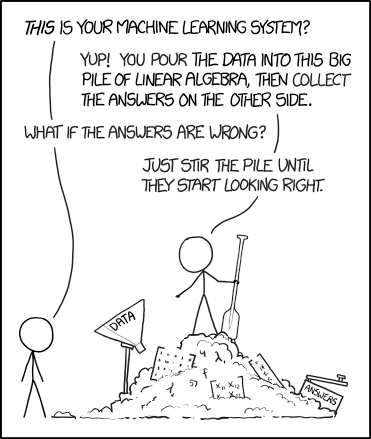
\includegraphics[height=0.65\textheight]{images/1838_machine_learning.png}
\vspace{2mm}

\textit{``You pour the data into this big pile of linear algebra, then collect the answers on the other side.''}
\bottomnote{XKCD \#1838 ``Machine Learning'' by Randall Munroe (CC BY-NC 2.5)}
\end{frame}

% --- Slide 3: Learning Objectives ---
\begin{frame}{What Will You Learn Today?}
\begin{compactlist}
\item \highlight{Analyze} why one-hot encoding fails for NLP tasks
\item \highlight{Evaluate} trade-offs between static and contextual embeddings
\item \highlight{Apply} cosine similarity to measure semantic closeness
\item \highlight{Design} an embedding-based sentiment classifier for financial text
\item \highlight{Critique} embedding approaches for specific finance use cases
\end{compactlist}
\bottomnote{Bloom's levels 4--5: Analyze, Evaluate, Apply, Design, Critique}
\end{frame}

% --- Slide 4: Table of Contents ---
\begin{frame}{Roadmap}
\tableofcontents
\bottomnote{From one-hot encoding to RAG: the complete embeddings journey}
\end{frame}

\section{The Problem}

% --- Slide 5: Why Can't Machines Read Text? ---
\begin{frame}{Why Can't Machines Read Text?}
\begin{compactlist}
\item \highlight{The problem:} text is categorical, not numeric --- models need numbers
\item An earnings call transcript has 10,000 words --- how do we feed that to a model?
\item \textbf{Sparse representation:} each word is an isolated symbol with no relationships
\item \textbf{High dimensionality:} vocabulary sizes of 50,000--100,000 are common
\item \textbf{No similarity:} ``bullish'' and ``optimistic'' look equally different as ``bullish'' and ``penguin''
\end{compactlist}
\bottomnote{The fundamental challenge: converting discrete symbols into continuous vectors}
\end{frame}

% =====================================================
% ACT 2: STATIC EMBEDDINGS (Slides 6--15)
% =====================================================
\section{Static Embeddings}

% --- Slide 6: One-Hot Encoding (MVF) ---
\begin{frame}{What Is One-Hot Encoding?}
\textbf{Motivate:} A vocabulary of 10,000 words means 10,000-dimensional sparse vectors.

\vspace{2mm}
\textbf{Visualize:}
\begin{center}
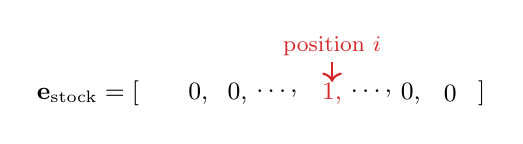
\begin{tikzpicture}[font=\small]
\node at (0,0) {$\mathbf{e}_{\text{stock}} = [$};
\node at (1.4,0) {$0,$};
\node at (1.9,0) {$0,$};
\node at (2.4,0) {$\ldots,$};
\node[text=mlred,font=\small\bfseries] at (3.1,0) {$1,$};
\node at (3.6,0) {$\ldots,$};
\node at (4.1,0) {$0,$};
\node at (4.6,0) {$0$};
\node at (5.0,0) {$]$};
\draw[->,mlred,thick] (3.1,0.4) -- (3.1,0.15);
\node[text=mlred,font=\footnotesize] at (3.1,0.6) {position $i$};
\end{tikzpicture}
\end{center}

\textbf{Formalize:} $\mathbf{e}_i \in \{0,1\}^{|V|}$ where $e_{ij} = 1$ iff $j = i$
\bottomnote{One-hot: simple but wasteful. No similarity between any two words.}
\end{frame}

% --- Slide 7: Distributional Hypothesis ---
\begin{frame}{What Does `Context' Tell Us About Meaning?}
\begin{compactlist}
\item \highlight{Distributional hypothesis:} ``You shall know a word by the company it keeps'' (Firth, 1957)
\item Finance: ``bullish'' appears near ``growth'', ``revenue'', ``upgrade''
\end{compactlist}

\vspace{3mm}
\begin{center}
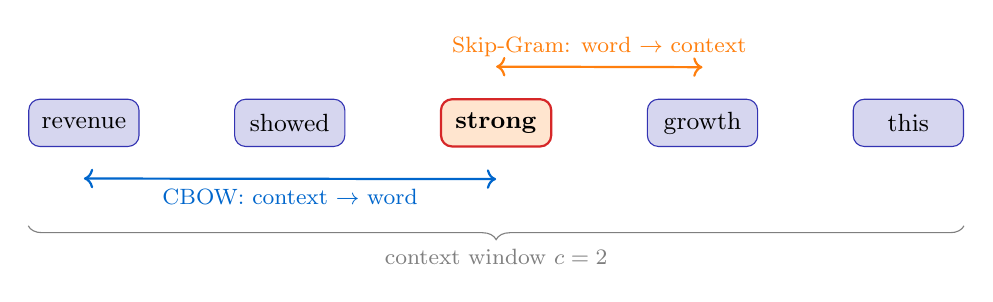
\begin{tikzpicture}[font=\small, node distance=1.2cm,
    word/.style={rectangle, rounded corners, draw=mlpurple, fill=mllavender4, minimum height=6mm, minimum width=14mm},
    center/.style={rectangle, rounded corners, draw=mlred, fill=mlorange!20, minimum height=6mm, minimum width=14mm, thick}]
  \node[word] (w1) {revenue};
  \node[word, right=of w1] (w2) {showed};
  \node[center, right=of w2] (wt) {\textbf{strong}};
  \node[word, right=of wt] (w3) {growth};
  \node[word, right=of w3] (w4) {this};

  \draw[<->,mlblue,thick] ([yshift=-4mm]w1.south) -- node[below,font=\footnotesize] {CBOW: context $\to$ word} ([yshift=-4mm]wt.south);
  \draw[<->,mlorange,thick] ([yshift=4mm]wt.north) -- node[above,font=\footnotesize] {Skip-Gram: word $\to$ context} ([yshift=4mm]w3.north);

  \draw[decorate,decoration={brace,amplitude=5pt,mirror},mlgray] ([yshift=-10mm]w1.south west) -- ([yshift=-10mm]w4.south east) node[midway,below=5pt,font=\footnotesize] {context window $c = 2$};
\end{tikzpicture}
\end{center}
\bottomnote{The distributional hypothesis: the foundation of all word embedding methods (Firth, 1957)}
\end{frame}

% --- Slide 8: Skip-Gram Architecture (chart-only) ---
\begin{frame}{How Does the Skip-Gram Network Look?}
\begin{center}

\includegraphics[width=0.65\textwidth]{08_skipgram_architecture/chart.pdf}
\end{center}
\begin{compactlist}
\item \textbf{Input:} one-hot vector $\mathbf{e}_w \in \mathbb{R}^{|V|}$, \textbf{Hidden:} embedding $\mathbf{v}_w = W^{\!\top}\mathbf{e}_w \in \mathbb{R}^d$
\item \textbf{Output:} context matrix $W'$ produces softmax over vocabulary
\end{compactlist}
\bottomnote{Skip-Gram: predict context words from the center word. Two embedding matrices: $W$ (input) and $W'$ (output).}
\end{frame}

% --- Slide 9: Skip-Gram Objective (MVF) ---
\begin{frame}{What Is the Skip-Gram Objective?}
\textbf{Motivate:} We want to maximize the probability of seeing the actual context words.

\vspace{1mm}
Finance example: predicting ``revenue'' appears near ``earnings''.

\vspace{2mm}
\textbf{Formalize:}
\small
\[
J = \frac{1}{T}\sum_{t=1}^{T}\sum_{\substack{-c \le j \le c \\ j\neq 0}} \log p(w_{t+j} \mid w_t)
\]
where $p(w_O \mid w_I) = \dfrac{\exp(\mathbf{v}'_{w_O}{}^{\!\top} \mathbf{v}_{w_I})}{\sum_{w=1}^{|V|}\exp(\mathbf{v}'_w{}^{\!\top} \mathbf{v}_{w_I})}$
\normalsize
\bottomnote{The softmax denominator sums over ALL words in the vocabulary --- this will be a problem.}
\end{frame}

% --- Slide 10: Full Softmax Intractable ---
\begin{frame}{Why Is Full Softmax Intractable?}
\begin{compactlist}
\item \highlight{$O(|V|)$ per update} for $V = 100{,}000+$ --- every gradient step touches the entire vocabulary
\item The denominator $\sum_{w=1}^{|V|}\exp(\mathbf{v}'_w{}^{\!\top}\mathbf{v}_{w_I})$ requires computing all dot products
\item \textbf{Two solutions:} hierarchical softmax (tree structure) and \highlight{negative sampling} (binary classification)
\end{compactlist}
\bottomnote{Computing the full softmax is the main computational bottleneck of Word2Vec.}
\end{frame}

% --- Slide 11: Negative Sampling (MVF) ---
\begin{frame}{How Does Negative Sampling Fix This?}
\textbf{Motivate:} Replace $V$-class softmax with $K+1$ binary classifiers.

\vspace{1mm}
\begin{columns}[T]
\begin{column}{0.55\textwidth}

\includegraphics[width=\textwidth]{10_negative_sampling/chart.pdf}
\end{column}
\begin{column}{0.42\textwidth}
\small
\textbf{Formalize:}
\vspace{1mm}

$J_{\text{NEG}} = \log\sigma(\mathbf{v}'_{w_O}{}^{\!\top} \mathbf{v}_{w_I})$

$+ \displaystyle\sum_{k=1}^{K}\mathbb{E}_{w_k \sim P_n}\!\left[\log\sigma(-\mathbf{v}'_{w_k}{}^{\!\top} \mathbf{v}_{w_I})\right]$

\vspace{2mm}
Push \highlight{positive pairs} together, push \highlight{negative pairs} apart.
\normalsize
\end{column}
\end{columns}
\bottomnote{Negative sampling: $O(K)$ instead of $O(|V|)$. Typically $K = 5$--$20$ negatives per positive pair.}
\end{frame}

% --- Slide 12: Sampling Algorithm ---
\begin{frame}{How Do We Sample Negative Words?}
\begin{columns}[T]
\begin{column}{0.55\textwidth}
\begin{algorithmic}[1]
\small
\STATE Initialize $W$, $W'$ randomly
\FOR{each word $w_t$ in corpus}
  \FOR{each context word $w_c$ in window}
    \STATE \textcolor{mlgreen}{\textbf{Positive:}} update $(w_t, w_c)$ to increase $\sigma$
    \FOR{$k = 1$ to $K$}
      \STATE Sample $w_n \sim P_n(w)$
      \STATE \textcolor{mlred}{\textbf{Negative:}} update $(w_t, w_n)$ to decrease $\sigma$
    \ENDFOR
  \ENDFOR
\ENDFOR
\end{algorithmic}
\end{column}
\begin{column}{0.42\textwidth}
\textbf{Noise distribution:}

\vspace{2mm}
$P_n(w) = \dfrac{f(w)^{3/4}}{\sum_{w'} f(w')^{3/4}}$

\vspace{3mm}
The $3/4$ exponent \highlight{upweights rare words} relative to their raw frequency.
\end{column}
\end{columns}
\bottomnote{The 3/4 exponent upweights rare words relative to their frequency (Mikolov et al., 2013).}
\end{frame}

% --- Slide 13: Embedding Space (chart-only) ---
\begin{frame}{What Does the Embedding Space Look Like?}
\begin{center}

\includegraphics[width=0.65\textwidth]{01_word_embedding_space/chart.pdf}
\end{center}
\begin{compactlist}
\item Similar words cluster together in the learned embedding space
\item Finance terms (stock, bond, equity) form a semantic neighborhood
\end{compactlist}
\bottomnote{t-SNE projection of 50-dimensional word vectors. Similar words cluster in embedding space.}
\end{frame}

% --- Slide 14: Cosine Similarity (MVF) ---
\begin{frame}{How Do We Measure Semantic Closeness?}
\textbf{Motivate:} Euclidean distance fails when vectors have different magnitudes.

\vspace{1mm}
\begin{columns}[T]
\begin{column}{0.48\textwidth}

\includegraphics[width=\textwidth]{02_similarity_heatmap/chart.pdf}
\end{column}
\begin{column}{0.48\textwidth}
\textbf{Formalize:}

\vspace{2mm}
$\text{cos}(\mathbf{a}, \mathbf{b}) = \dfrac{\mathbf{a} \cdot \mathbf{b}}{\|\mathbf{a}\|\;\|\mathbf{b}\|}$

\vspace{3mm}
\textbf{Finance examples:}
\begin{compactlist}
\item $\cos(\text{bullish}, \text{positive}) = 0.82$
\item $\cos(\text{bullish}, \text{negative}) = -0.31$
\end{compactlist}
\end{column}
\end{columns}
\bottomnote{Cosine similarity: range $[-1, 1]$. Direction matters, not magnitude.}
\end{frame}

% --- Slide 15: Word Analogies ---
\begin{frame}{Can We Do Arithmetic with Words?}
\begin{columns}[T]
\begin{column}{0.55\textwidth}

\includegraphics[width=\textwidth]{11_word_analogy_arithmetic/chart.pdf}
\end{column}
\begin{column}{0.42\textwidth}
\textbf{Classic:}

\vspace{1mm}
$\mathbf{v}_{\text{king}} - \mathbf{v}_{\text{man}} + \mathbf{v}_{\text{woman}} \approx \mathbf{v}_{\text{queen}}$

\vspace{3mm}
\textbf{Finance:}

\vspace{1mm}
$\mathbf{v}_{\text{stock}} - \mathbf{v}_{\text{equity}} + \mathbf{v}_{\text{debt}} \approx \mathbf{v}_{\text{bond}}$

\vspace{3mm}
Vector arithmetic captures \highlight{relational structure} in embedding space.
\end{column}
\end{columns}
\bottomnote{Vector arithmetic captures relational structure. Success rate: 40--70\% (Levy \& Goldberg, 2014).}
\end{frame}

% =====================================================
% ACT 3: BEYOND WORD2VEC (Slides 16--18)
% =====================================================
\section{Beyond Word2Vec}

% --- Slide 16: GloVe (MVF) ---
\begin{frame}{What If We Use Global Statistics Instead?}
\textbf{Motivate:} Word2Vec only uses local context windows. \highlight{GloVe} uses global co-occurrence statistics.

\vspace{2mm}
\textbf{Formalize:}
\small
\[
J = \sum_{i,j=1}^{|V|} f(X_{ij})\!\left(\mathbf{w}_i^{\!\top} \tilde{\mathbf{w}}_j + b_i + \tilde{b}_j - \log X_{ij}\right)^{\!2}
\]
\normalsize

where $X_{ij}$ = co-occurrence count and the weighting function is:

\vspace{1mm}
$f(x) = \min\!\left((x/x_{\max})^{0.75},\; 1\right)$

\vspace{2mm}
\begin{compactlist}
\item Combines count-based (LSA) and prediction-based (Word2Vec) advantages
\item Weighting caps frequent pairs, upweights informative rare pairs
\end{compactlist}
\bottomnote{GloVe: combines global co-occurrence statistics with embedding learning (Pennington et al., 2014).}
\end{frame}

% --- Slide 17: FastText (MVF) ---
\begin{frame}{How Do We Handle Unknown Words?}
\textbf{Motivate:} The OOV problem --- ``bullish'' unseen if only ``bull'' was trained.

\vspace{2mm}
\textbf{Example:} ``bullish'' $\to$ [\texttt{<bu}, \texttt{bul}, \texttt{ull}, \texttt{lli}, \texttt{lis}, \texttt{ish}, \texttt{sh>}]

\vspace{3mm}
\textbf{Formalize:}
\[
\mathbf{v}_w = \sum_{g \in \mathcal{G}(w)} \mathbf{z}_g
\]

where $\mathcal{G}(w)$ is the set of character n-grams (typically $n = 3$--$6$).

\vspace{2mm}
\begin{compactlist}
\item Any new word can be represented via its subword pieces
\item Captures morphology: ``un-'' prefix, ``-tion'' suffix carry meaning
\end{compactlist}
\bottomnote{FastText: character n-grams solve the OOV problem and capture morphology (Bojanowski et al., 2017).}
\end{frame}

% --- Slide 18: Hyperparameters ---
\begin{frame}{How Do Hyperparameters Affect Embeddings?}
\begin{columns}[T]
\begin{column}{0.55\textwidth}

\includegraphics[width=\textwidth]{top10_12_context_window/chart.pdf}
\end{column}
\begin{column}{0.42\textwidth}
\begin{compactlist}
\item \textbf{Small window} ($c = 2$): captures syntactic patterns (POS, grammar)
\item \textbf{Large window} ($c = 10$): captures semantic/topical similarity
\item \textbf{Dimensions:} 50--300 typical; diminishing returns beyond 300
\end{compactlist}
\end{column}
\end{columns}
\bottomnote{Window size and dimensions are the two most important hyperparameters for static embeddings.}
\end{frame}

% =====================================================
% ACT 4: FROM STATIC TO CONTEXTUAL (Slides 19--27)
% =====================================================
\section{Contextual Embeddings}

% --- Slide 19: Polysemy Problem ---
\begin{frame}{What Happens When Words Have Multiple Meanings?}
\begin{columns}[c]
\begin{column}{0.55\textwidth}

\includegraphics[width=\textwidth]{17_static_vs_contextual_embedding/chart.pdf}
\end{column}
\begin{column}{0.42\textwidth}
\begin{compactlist}
\item ``Bank'' = financial institution OR riverbank
\item ``Interest'' = financial vs.\ personal
\item Static: \highlight{one vector per word}
\end{compactlist}
\end{column}
\end{columns}
\bottomnote{The polysemy problem: static embeddings assign one vector per word regardless of context.}
\end{frame}

% --- Slide 20: Tokenization (BPE + WordPiece) ---
\begin{frame}{How Do Models Split Text into Tokens?}
\textbf{Example:} ``unaffordable'' $\to$ [\texttt{un}, \texttt{\#\#afford}, \texttt{\#\#able}]

\vspace{3mm}
\small
\begin{columns}[T]
\begin{column}{0.48\textwidth}
\textbf{BPE} (GPT family):

$\text{merge} = \arg\max_{(a,b)} \text{count}(ab)$

\vspace{1mm}
Frequency-based: merge the most common adjacent pair.
\end{column}
\begin{column}{0.48\textwidth}
\textbf{WordPiece} (BERT family):

$\text{merge} = \arg\max_{(a,b)} \dfrac{\text{freq}(ab)}{\text{freq}(a) \cdot \text{freq}(b)}$

\vspace{1mm}
Likelihood-based: merge pairs that most increase corpus likelihood.
\end{column}
\end{columns}
\normalsize

\vspace{3mm}
\begin{compactlist}
\item Both reduce vocabulary to 30K--50K tokens while preserving subword meaning
\item No more OOV --- any word can be split into known subword tokens
\end{compactlist}
\bottomnote{BPE: frequency-based merging. WordPiece: likelihood-ratio merging. Both reduce vocabulary while keeping subword meaning.}
\end{frame}

% --- Slide 21: Positional Encoding (MVF) ---
\begin{frame}{How Do Transformers Know Word Order?}
\textbf{Motivate:} Transformers process all tokens in parallel --- they need position information injected.

\vspace{3mm}
\textbf{Formalize:}
\[
PE_{(pos,2i)} = \sin\!\left(\frac{pos}{10000^{2i/d}}\right), \quad PE_{(pos,2i+1)} = \cos\!\left(\frac{pos}{10000^{2i/d}}\right)
\]

\vspace{2mm}
\begin{compactlist}
\item Each position gets a \highlight{unique frequency signature} --- no two positions are alike
\item Sinusoidal encoding allows the model to attend to relative positions
\item Added directly to token embeddings: $\mathbf{x}_i = \mathbf{e}_{\text{token}} + \mathbf{e}_{\text{pos}}$
\end{compactlist}
\bottomnote{Sinusoidal position encoding: each position gets a unique frequency signature (Vaswani et al., 2017).}
\end{frame}

% --- Slide 22: Attention (MVF) ---
\begin{frame}{Which Words Should I Pay Attention To?}
\textbf{Motivate:} Q/K/V analogy --- Query = what I'm looking for, Key = what I offer, Value = what I contain.

\vspace{3mm}
\textbf{The key formula:}
\[
\text{Attention}(Q,K,V) = \text{softmax}\!\left(\frac{QK^{\!\top}}{\sqrt{d_k}}\right)V
\]

\vspace{2mm}
\begin{compactlist}
\item $QK^{\!\top}$: how much should each token attend to every other token?
\item $\sqrt{d_k}$: scaling prevents softmax from saturating for large $d_k$
\item Result: each token is a \highlight{weighted sum} of all value vectors
\end{compactlist}
\bottomnote{Scaled dot-product attention: the core mechanism of all transformer models (Vaswani et al., 2017).}
\end{frame}

% --- Slide 23: Multi-Head Attention (MVF) ---
\begin{frame}{Why Use Multiple Attention Heads?}
\textbf{Motivate:} One head captures syntax, another captures semantics --- multiple heads in parallel.

\vspace{3mm}
\textbf{Formalize:}
\[
\text{MultiHead}(Q,K,V) = \text{Concat}(h_1,\ldots,h_H)\,W^O
\]
where $h_i = \text{Attention}(QW_i^Q,\; KW_i^K,\; VW_i^V)$

\vspace{2mm}
\begin{compactlist}
\item Each head projects Q, K, V to dimension $d_k = d_{\text{model}} / H$
\item BERT uses $H = 12$ heads; GPT-3 uses $H = 96$ heads
\item Concatenated outputs are projected back to $d_{\text{model}}$
\end{compactlist}
\bottomnote{Multi-head attention: $H$ parallel attention functions capture different relationship types.}
\end{frame}

% --- Slide 24: Transformer Block (TikZ) ---
\begin{frame}{What Does a Transformer Block Look Like?}
\begin{center}
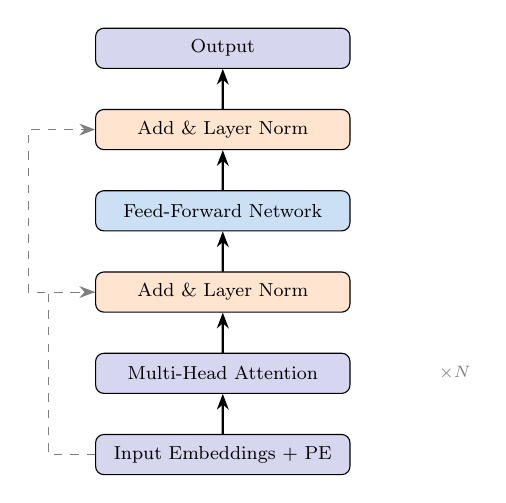
\begin{tikzpicture}[scale=0.85, every node/.style={transform shape},
    block/.style={rectangle, rounded corners=3pt, draw, minimum width=38mm, minimum height=6mm, font=\footnotesize, align=center},
    arr/.style={-{Stealth[length=2mm]}, thick},
    skip/.style={-{Stealth[length=2mm]}, dashed, mlgray},
    node distance=6mm
]
  \node[block, fill=mllavender4] (input) {Input Embeddings + PE};
  \node[block, fill=mlpurple!20, above=of input] (attn) {Multi-Head Attention};
  \node[block, fill=mlorange!20, above=of attn] (norm1) {Add \& Layer Norm};
  \node[block, fill=mlblue!20, above=of norm1] (ffn) {Feed-Forward Network};
  \node[block, fill=mlorange!20, above=of ffn] (norm2) {Add \& Layer Norm};
  \node[block, fill=mllavender4, above=of norm2] (output) {Output};
  \draw[arr] (input) -- (attn);
  \draw[arr] (attn) -- (norm1);
  \draw[arr] (norm1) -- (ffn);
  \draw[arr] (ffn) -- (norm2);
  \draw[arr] (norm2) -- (output);
  \draw[skip] (input.west) -- ++(-7mm,0) |- (norm1.west);
  \draw[skip] (norm1.west) -- ++(-10mm,0) |- (norm2.west);
  \node[font=\scriptsize, text=mlgray, right=12mm of attn] {$\times N$};
\end{tikzpicture}
\end{center}
\bottomnote{The transformer block: the building unit repeated $N$ times in BERT (12$\times$) and GPT (12--96$\times$).}
\end{frame}

% --- Slide 25: BERT MLM (MVF) ---
\begin{frame}{How Does BERT Read in Both Directions?}
\textbf{Motivate:} GPT reads left-to-right only. BERT masks random words and predicts them from \highlight{both sides}.

\vspace{3mm}
\textbf{Formalize --- Masked Language Modeling:}
\[
\mathcal{L}_{\text{MLM}} = -\sum_{i \in \mathcal{M}} \log p(x_i \mid \mathbf{x}_{\backslash\mathcal{M}})
\]

where $\mathcal{M}$ = set of masked positions (15\% of tokens).

\vspace{2mm}
\begin{compactlist}
\item Example: ``The [MASK] reported strong earnings'' $\to$ predict ``company''
\item Bidirectional context: uses both left and right words to predict
\item Pre-trained on BookCorpus + Wikipedia (3.3B words)
\end{compactlist}
\bottomnote{BERT: Masked Language Modeling + Next Sentence Prediction. Pre-trained on BookCorpus + Wikipedia.}
\end{frame}

% --- Slide 26: Fine-Tuning for Classification (MVF) ---
\begin{frame}{How Do We Fine-Tune for Classification?}
\textbf{Motivate:} The \texttt{[CLS]} token representation feeds a linear layer for downstream tasks.

\vspace{1mm}
Finance: classifying an earnings call as positive/negative.

\vspace{3mm}
\textbf{Formalize:}
\[
\hat{y}_c = \text{softmax}(\mathbf{W}\,\mathbf{h}_{[\text{CLS}]} + \mathbf{b})_c, \qquad \mathcal{L} = -\sum_{c=1}^{C} y_c \log(\hat{y}_c)
\]

\vspace{2mm}
\begin{compactlist}
\item \textbf{Pre-train} on large unlabeled corpus (expensive, done once)
\item \textbf{Fine-tune} on small labeled dataset (cheap, task-specific)
\item Only the classification head + top BERT layers are updated
\end{compactlist}
\bottomnote{Cross-entropy loss on the [CLS] representation: the standard approach for text classification.}
\end{frame}

% --- Slide 27: BERT vs GPT Comparison ---
\begin{frame}{When Should You Use BERT vs GPT?}
\begin{center}
\small
\begin{tabular}{@{}l l l@{}}
\toprule
\textbf{Property} & \textbf{BERT} & \textbf{GPT} \\
\midrule
Direction & Bidirectional & Left-to-right \\
Pre-training & MLM + NSP & Next token prediction \\
Best for & Classification, NER, QA & Text generation \\
Finance use & Sentiment, entity extraction & Report generation \\
Parameters & 110M (base) / 340M (large) & 117M (1) to 175B (3) \\
\bottomrule
\end{tabular}
\normalsize
\end{center}

\vspace{2mm}
\begin{compactlist}
\item \highlight{BERT for understanding}, \highlight{GPT for generation}
\item Both use the same transformer architecture --- the difference is the training objective
\item Modern LLMs (GPT-4, Claude) use decoder-only architecture at massive scale
\end{compactlist}
\bottomnote{BERT for understanding, GPT for generation. Both use the same transformer architecture.}
\end{frame}

% =====================================================
% ACT 5: FINANCE APPLICATIONS (Slides 28--35)
% =====================================================
\section{Finance Applications}

% --- Slide 28: FinBERT ---
\begin{frame}{Why Does General BERT Fail on Financial Text?}
\begin{columns}[T]
\begin{column}{0.55\textwidth}

\includegraphics[width=\textwidth]{16_finbert_sentiment_bars/chart.pdf}
\end{column}
\begin{column}{0.42\textwidth}
\begin{compactlist}
\item ``Liability'' = negative in general English, \highlight{neutral in finance}
\item ``Volatile'' = negative generally, descriptive in markets
\item FinBERT: BERT fine-tuned on financial news, earnings calls, analyst reports
\end{compactlist}
\end{column}
\end{columns}
\bottomnote{FinBERT: BERT fine-tuned on financial text achieves 87\% accuracy on sentiment (Araci, 2019).}
\end{frame}

% --- Slide 29: Sentiment Pipeline (TikZ) ---
\begin{frame}{How Does the Full Sentiment Pipeline Work?}
\begin{center}
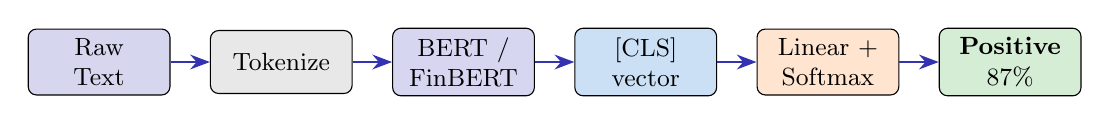
\begin{tikzpicture}[
    box/.style={rectangle, rounded corners=3pt, draw, minimum height=8mm, minimum width=18mm, font=\small, align=center},
    arr/.style={-{Stealth[length=2.5mm]}, thick, mlpurple},
    node distance=5mm
]
  \node[box, fill=mllavender4] (raw) {Raw\\Text};
  \node[box, fill=midgray!30, right=of raw] (tok) {Tokenize};
  \node[box, fill=mlpurple!20, right=of tok] (bert) {BERT /\\FinBERT};
  \node[box, fill=mlblue!20, right=of bert] (cls) {[CLS]\\vector};
  \node[box, fill=mlorange!20, right=of cls] (lin) {Linear +\\Softmax};
  \node[box, fill=mlgreen!20, right=of lin] (out) {\textbf{Positive}\\87\%};

  \draw[arr] (raw) -- (tok);
  \draw[arr] (tok) -- (bert);
  \draw[arr] (bert) -- (cls);
  \draw[arr] (cls) -- (lin);
  \draw[arr] (lin) -- (out);
\end{tikzpicture}
\end{center}

\vspace{3mm}
\begin{compactlist}
\item Finance running example: ``Q3 revenue exceeded expectations with 12\% growth''
\item The \texttt{[CLS]} token aggregates the full sentence meaning into one vector
\item Linear layer maps 768-dim vector to 3 classes: positive / negative / neutral
\end{compactlist}
\bottomnote{End-to-end sentiment classification: text $\to$ tokens $\to$ BERT $\to$ [CLS] $\to$ softmax $\to$ label.}
\end{frame}

% --- Slide 30: Sentence-BERT (MVF) ---
\begin{frame}{How Do We Get Sentence-Level Embeddings?}
\textbf{Motivate:} BERT gives token-level embeddings, not sentence-level. Sentence-BERT uses a \highlight{siamese network}.

\vspace{2mm}
\begin{center}
\begin{tikzpicture}[
    box/.style={rectangle, rounded corners=3pt, draw, minimum height=7mm, minimum width=20mm, font=\small, align=center},
    arr/.style={-{Stealth[length=2mm]}, thick},
    node distance=6mm
]
  % Left tower
  \node[box, fill=mlpurple!20] (bert1) {BERT};
  \node[box, fill=mlblue!20, above=of bert1] (pool1) {Mean Pool};
  \node[font=\small, below=of bert1] (s1) {Sentence A};

  % Right tower
  \node[box, fill=mlpurple!20, right=30mm of bert1] (bert2) {BERT};
  \node[box, fill=mlblue!20, above=of bert2] (pool2) {Mean Pool};
  \node[font=\small, below=of bert2] (s2) {Sentence B};

  % Shared weights
  \draw[<->, dashed, mlgray] (bert1.east) -- node[above, font=\footnotesize] {shared} (bert2.west);

  % Arrows
  \draw[arr] (s1) -- (bert1);
  \draw[arr] (bert1) -- (pool1);
  \draw[arr] (s2) -- (bert2);
  \draw[arr] (bert2) -- (pool2);

  % Cosine
  \node[box, fill=mlorange!20, above=16mm of $(pool1)!0.5!(pool2)$] (cos) {$\cos(\mathbf{u}, \mathbf{v})$};
  \draw[arr] (pool1) -- (cos);
  \draw[arr] (pool2) -- (cos);
\end{tikzpicture}
\end{center}

\vspace{1mm}
$\mathcal{L} = \frac{1}{N}\sum_{i=1}^{N}\!\left(\cos(\mathbf{u}_i, \mathbf{v}_i) - y_i\right)^{\!2}$ \quad where $y_i \in [-1, 1]$
\bottomnote{Sentence-BERT: cosine similarity MSE loss for contrastive sentence learning (Reimers \& Gurevych, 2019).}
\end{frame}

% --- Slide 31: SEC Filing Similarity ---
\begin{frame}{Can We Detect Changes in SEC Filings?}
\begin{compactlist}
\item Compare 10-K filings year-over-year using \highlight{document embeddings}
\item If $\cos(\mathbf{d}_{2024}, \mathbf{d}_{2025}) < 0.85$, flag for manual review
\item Material changes in risk factors, revenue recognition, or legal proceedings are detectable
\end{compactlist}

\vspace{3mm}
\begin{center}
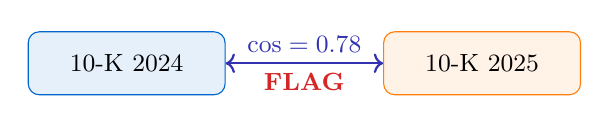
\begin{tikzpicture}[font=\small]
  \node[rectangle, rounded corners, draw=mlblue, fill=mlblue!10, minimum width=25mm, minimum height=8mm] (d1) {10-K 2024};
  \node[rectangle, rounded corners, draw=mlorange, fill=mlorange!10, minimum width=25mm, minimum height=8mm, right=20mm of d1] (d2) {10-K 2025};
  \draw[<->, thick, mlpurple] (d1) -- node[above] {$\cos = 0.78$} node[below, text=mlred] {\textbf{FLAG}} (d2);
\end{tikzpicture}
\end{center}
\bottomnote{Document similarity via cosine: a simple but powerful compliance monitoring tool.}
\end{frame}

% --- Slide 32: RAG Pipeline (chart-only) ---
\begin{frame}{How Does RAG Connect Embeddings to LLMs?}
\begin{center}

\includegraphics[width=0.65\textwidth]{14_rag_pipeline_flow/chart.pdf}
\end{center}
\begin{compactlist}
\item Query $\to$ embed $\to$ search vector DB $\to$ retrieve top-$k$ $\to$ augment prompt $\to$ generate
\item Grounds LLM responses in \highlight{factual, up-to-date} documents --- reduces hallucination
\end{compactlist}
\bottomnote{RAG: Retrieval-Augmented Generation. Combines embedding search with LLM generation.}
\end{frame}

% --- Slide 33: Named Entity Recognition ---
\begin{frame}{What Entities Can We Extract from Financial Text?}
\begin{compactlist}
\item \textbf{Tickers:} AAPL, MSFT, TSLA --- link mentions to structured databases
\item \textbf{Monetary amounts:} \$2.4B revenue, \EUR{}500M write-down
\item \textbf{Dates \& events:} ``Q3 2025 earnings'', ``Fed meeting March 19''
\end{compactlist}

\vspace{3mm}
\begin{center}
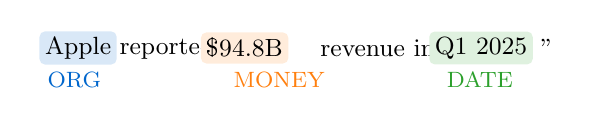
\begin{tikzpicture}[font=\small]
  \node[anchor=west] at (0,0) {``};
  \node[anchor=west, fill=mlblue!15, rounded corners=2pt, inner sep=2pt] at (0.15,0) {Apple};
  \node[anchor=west] at (1.05,0) {reported};
  \node[anchor=west, fill=mlorange!15, rounded corners=2pt, inner sep=2pt] at (2.2,0) {\$94.8B};
  \node[anchor=west] at (3.6,0) {revenue in};
  \node[anchor=west, fill=mlgreen!15, rounded corners=2pt, inner sep=2pt] at (5.1,0) {Q1 2025};
  \node[anchor=west] at (6.4,0) {''};

  \node[font=\footnotesize, text=mlblue] at (0.6,-0.4) {ORG};
  \node[font=\footnotesize, text=mlorange] at (3.2,-0.4) {MONEY};
  \node[font=\footnotesize, text=mlgreen] at (5.75,-0.4) {DATE};
\end{tikzpicture}
\end{center}

\vspace{2mm}
BERT + token classification head: predict B-ORG, I-ORG, B-MONEY, etc.\ per token.
\bottomnote{Named Entity Recognition: extract structured data from unstructured financial text.}
\end{frame}

% --- Slide 34: Trading Signals ---
\begin{frame}{Can Embeddings Generate Trading Signals?}
\begin{compactlist}
\item News sentiment $\to$ daily feature vector $\to$ ML model $\to$ buy/sell signal
\item Aggregate across all articles for a given day and ticker:
\end{compactlist}

\vspace{2mm}
\[
s_t = \frac{1}{N}\sum_{i=1}^{N}\text{sentiment}(\text{article}_i) \cdot \text{relevance}(\text{article}_i)
\]

\vspace{2mm}
\begin{compactlist}
\item \highlight{Walk-forward validation} required --- no peeking at future data
\item Combine with price features, volume, and technical indicators
\end{compactlist}
\bottomnote{Sentiment-based trading signals: aggregate news embeddings into daily features for ML models.}
\end{frame}

% --- Slide 35: Decision Table ---
\begin{frame}{Which Embedding Should You Choose?}
\begin{center}
\small
\begin{tabular}{@{}l l l@{}}
\toprule
\textbf{Method} & \textbf{Best For} & \textbf{Limitation} \\
\midrule
One-Hot & Tiny vocab, baseline & No similarity \\
Word2Vec / GloVe & Static, fast, large corpus & No polysemy \\
FastText & Morphologically rich, OOV & Still static \\
BERT & Context-dependent, classification & Slow, 512 tokens \\
Sentence-BERT & Document comparison & Needs fine-tuning \\
FinBERT & Financial text & Domain-specific only \\
\bottomrule
\end{tabular}
\normalsize
\end{center}

\vspace{2mm}
\begin{compactlist}
\item Start with the \highlight{simplest method that works}
\item Upgrade when you have evidence it will improve results
\item Always benchmark against a bag-of-words baseline
\end{compactlist}
\bottomnote{Start with the simplest method that works. Upgrade when you have evidence it will improve results.}
\end{frame}

% =====================================================
% ACT 6: WRAP-UP (Slides 36--39) --- ZONE 3
% =====================================================
\section{Wrap-Up}

% --- Slide 36: Key Takeaways ---
\begin{frame}{What Are the Key Takeaways?}
\begin{compactlist}
\item \highlight{Map} discrete text to continuous vectors with embeddings
\item \highlight{Capture} distributional semantics with Word2Vec / GloVe
\item \highlight{Add context} via transformer attention mechanisms
\item \highlight{Specialize} for finance with FinBERT and domain fine-tuning
\item \highlight{Connect} embeddings to LLMs via RAG for grounded generation
\end{compactlist}
\bottomnote{Five ideas that changed NLP: dense vectors, distributional learning, attention, fine-tuning, retrieval.}
\end{frame}

% --- Slide 37: Key Terms ---
\begin{frame}{Key Terms}
\begin{multicols}{2}
\begin{compactlist}
\item \textbf{Embedding} --- dense vector representing a discrete symbol
\item \textbf{One-Hot} --- sparse binary vector, one dimension per word
\item \textbf{Skip-Gram} --- predict context words from center word
\item \textbf{Cosine Similarity} --- direction-based similarity in $[-1, 1]$
\item \textbf{Attention} --- weighted sum using query--key--value
\item \textbf{BERT} --- bidirectional transformer, masked LM pre-training
\item \textbf{Fine-Tuning} --- adapt pre-trained model to downstream task
\item \textbf{RAG} --- retrieval-augmented generation for grounded LLM output
\end{compactlist}
\end{multicols}
\bottomnote{Master these 8 terms and you can discuss embeddings with any NLP practitioner.}
\end{frame}

% --- Slide 38: Exercises ---
\begin{frame}{What Should You Try Next?}
\begin{enumerate}
\setlength{\itemsep}{4pt}
\item Load pre-trained Word2Vec vectors and find the 10 nearest neighbors to ``inflation''
\item Compute cosine similarity between ``bullish'' and ``bearish'' --- is it positive or negative?
\item Use FinBERT to classify 5 financial headlines as positive / negative / neutral
\end{enumerate}

\vspace{3mm}
\begin{center}
\textcolor{mlblue}{\textbf{Colab notebook:}} \url{https://colab.research.google.com/}

\vspace{1mm}
\textit{See the L06 Colab notebook for starter code and pre-loaded data.}
\end{center}
\bottomnote{Hands-on: the best way to learn embeddings is to build with them. See the L06 Colab notebook.}
\end{frame}

% --- Slide 39: Closing Comic ---
\begin{frame}{From One-Hot to RAG: Journey Complete}
\centering
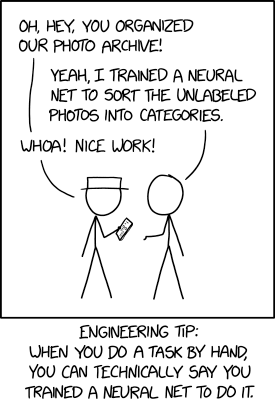
\includegraphics[height=0.55\textheight]{images/2173_trained_a_neural_net.png}

\vspace{2mm}
\textit{``I trained a neural net to identify the most important part of any image, and it says it's this neural net.''}
\bottomnote{XKCD \#2173 by Randall Munroe (CC BY-NC 2.5). From one-hot to RAG: the journey is complete!}
\end{frame}

\end{document}
